\chapter{Anwendung des Frameworks auf jadice flow}
\label{chap:anwendung}

In diesem Kapitel wird ein Architektur-Refactoring am Produkt \emph{jadice flow} geplant und in theoretischer Ebene durchgeführt.
Dazu wird das \gls{mmf} benutzt, das in \cref{sec:mmf} beschrieben wird.
Unterteilt ist der Prozess in drei Phasen, deren Durchführung im Folgenden beschrieben wird.

\section{Phase 1 - Architekturreview}

In dieser Phase wurde in einer Fokusgruppe ein Architekturreview nach \Citet{SVAHNBERG20071893} wie in \cref{sec:methodik-architekturreview} beschrieben durchgeführt.
Teil dieser Gruppe waren vier Softwareentwickler beziehungsweise -Architekten, der \acrlong{po} und ich selbst in der Rolle des Moderators.
Durch die ebenfalls in \cref{sec:methodik-architekturreview} beschriebenen Veränderungen an der Methodik von \Citet{SVAHNBERG20071893} wurde auch der geplante Zeitrahmen dieser Fokusgruppe auf lediglich 2 Stunden reduziert. Das liegt vor allem daran, dass die letzten Phasen nicht nötig waren, aber auch daran, dass alle Teilnehmer bereits vertraut mit dem Produkt und der Architektur und Funktionsweise des Systems waren. 
Demnach konnte nach einer kurzen Einleitung in die verwendete Methodik sofort mit Schritt 2, dem Ordnen der \glspl{qa} nach Wichtigkeit gestartet werden.
Dafür wurde 
% Dabei handelt es sich um eine Architekturbewertungsmethode, die auf Szenarien-basierten Methoden wie \gls{saam} (\Citet{saam}) und \gls{atam} (\Citet{kazman_2000}) aufbaut.
% Stakeholder definieren gemeinsam gewünschte Szenarien und ordnen diesen \glspl{qa} zu.
% Außerdem wird den verschiedenen Szenarien jeweils ein Grad der Schwierigkeit und ein Grad der Wichtigkeit zugewiesen.
% Die resultierenden Szenarien können in den \gls{arh} eingegeben werden.

Das Ergebnis dieser Fokusgruppe sind die Szenarien, in der \cref{tab:scenarios} zu sehen sind.

\begin{landscape}
	\begin{figure}
		\centering
		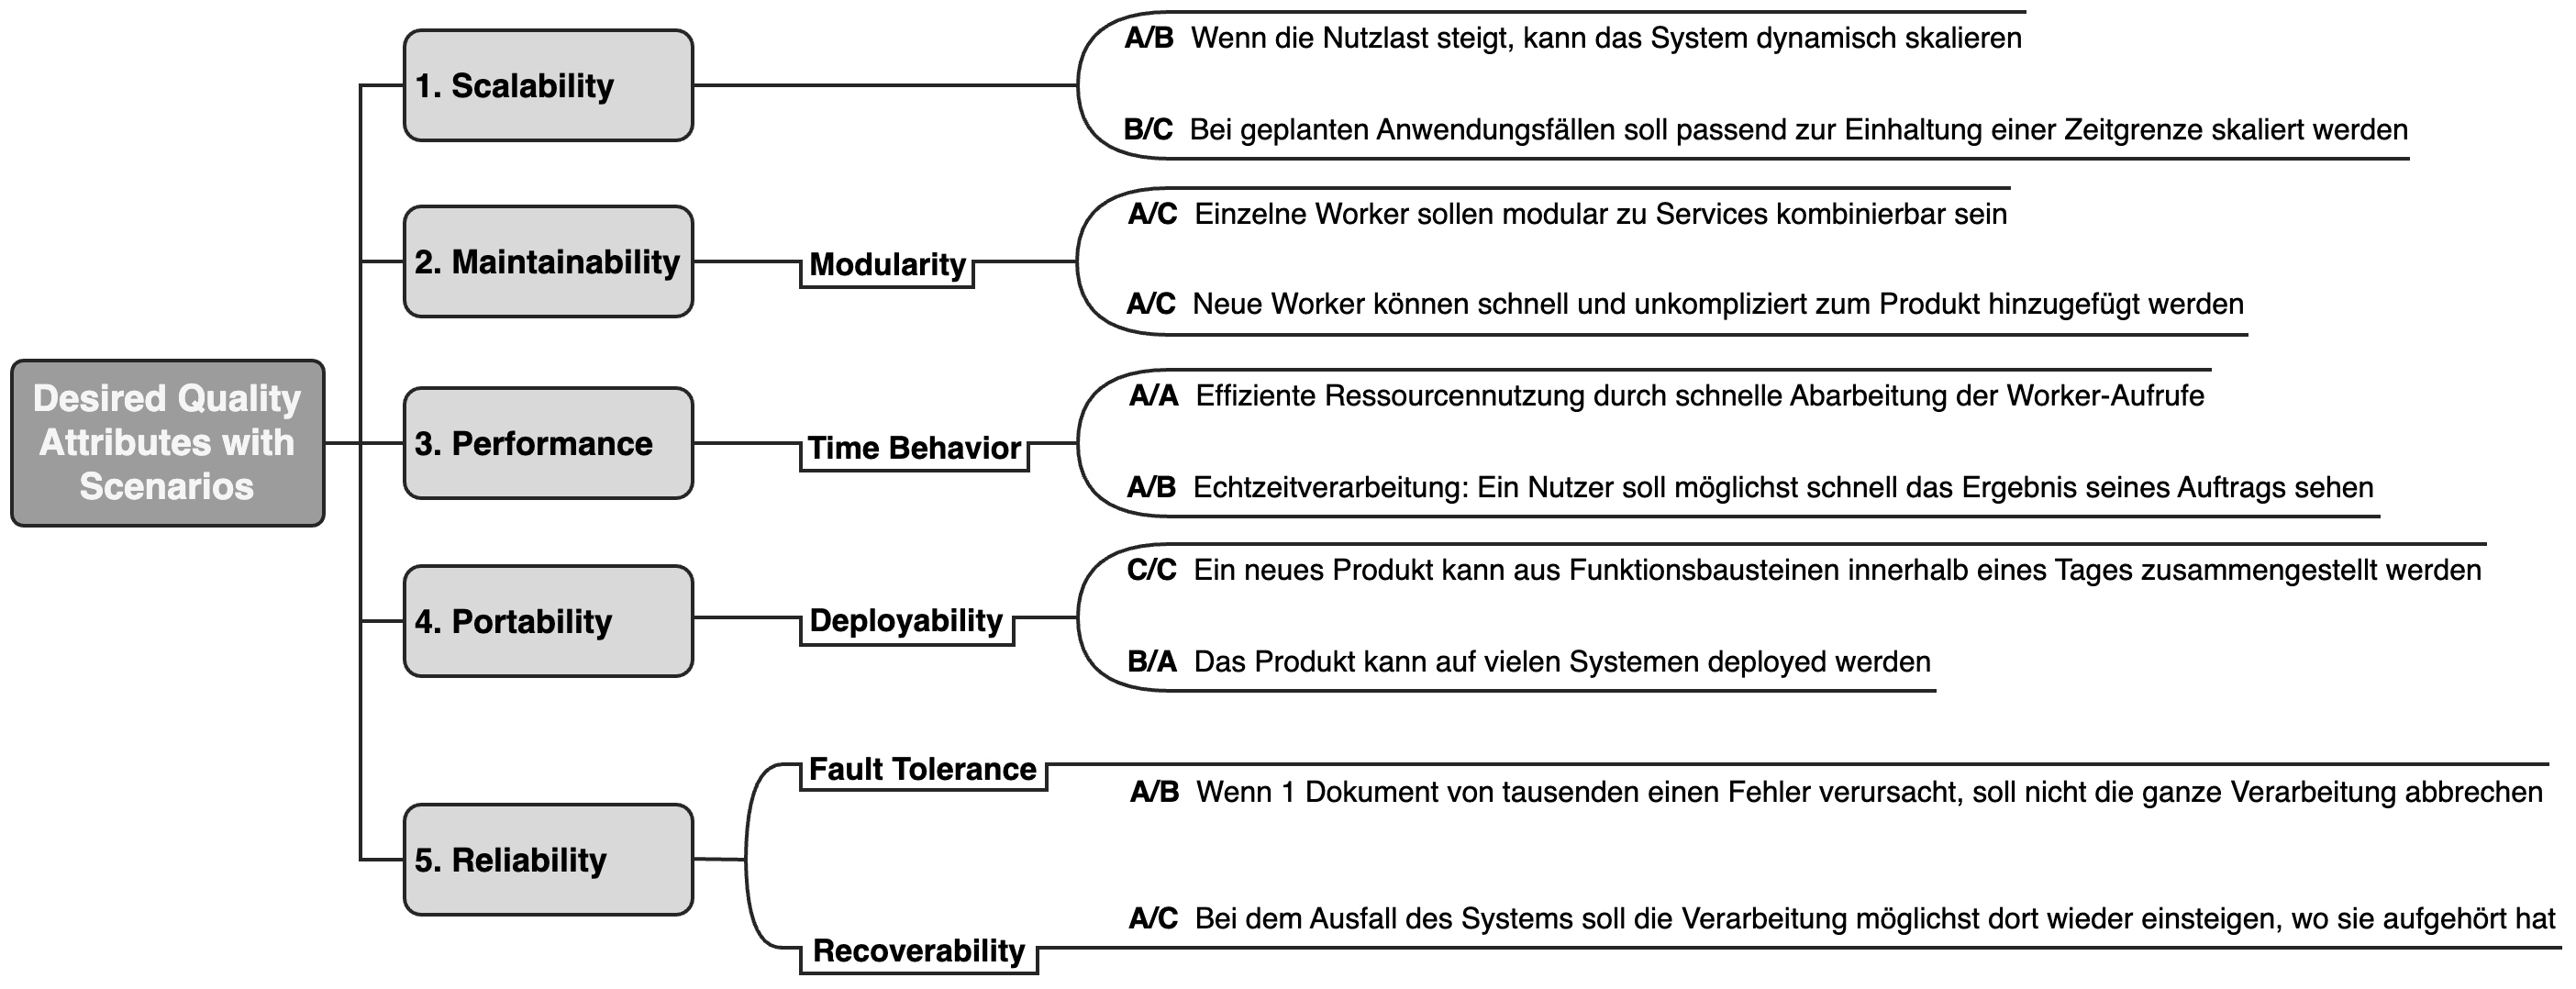
\includegraphics[width=1.5\textwidth]{scenarios.drawio}
		\caption[Utility Tree mit im Architekturreview ermittelten Qualitätsanforderungen und Szenarien]{
			Der Utility Tree mit Szenarien, die aus dem in Phase 1 durchgeführten Architekturreview resultieren.
			Von links nach rechts enthält der Baum folgende Elementarten: [1] Wurzel (ohne Bedeutung), [2] \gls{qa}, [3] Subattribut, [4] Beurteilung des Szenarios hinsichtlich Wichtigkeit und technischer Schwierigkeit, [5] Szenariobeschreibung.
		}
		\label{fig:scenarios}
	\end{figure}
\end{landscape}

Wie man in diesem Utility Tree sehen kann, sind die Szenarien nur mit jeweils einem \gls{qa} beziehungsweise Subattribut assoziiert.
Da realistischer Weise die meisten Szenarien allerdings mehrere \glspl{qa} beinhalten, wurden an einem zweiten Termin die Szenarien erneut betrachtet und diskutiert, welche weiteren \glspl{qa} sinnvoll hinzugefügt werden sollten.
Die resultierenden Assoziationen sind in der \cref{tab:scenarios} zu sehen.

\begin{table}
	\centering
	\begin{tabular}{ m{2,5cm} m{6cm} m{0.7cm} m{2,5cm} p{0.7cm} }
		\toprule
		\textbf{Name} & \textbf{Beschreibung} & \textbf{W/S} & \textbf{\glspl{qa}} & \textbf{MS} \\
		\midrule
		Dynamische Skalierbarkeit & Wenn die Nutzlast steigt, kann das System dynamisch skalieren & A/B & Scalability, Resource Utilization, Adaptability, Execution Cost & \advantage \\ \hline
		Statische Skalierbarkeit & Bei geplanten Anwendungsfällen soll passend zur Einhaltung einer Zeitgrenze skaliert werden & B/C & Scalability, Resource Utilization, Time Behavior & \advantage \\  \hline
		 Jobtemplates& Einzelne Worker sollen modular zu Services kombinierbar sein & A/C & Modularity, Reusability & - \\ \hline
		 Neue Worker& Neue Worker können schnell und unkompliziert zum Produkt hinzugefügt werden & A/C & Modularity, Reusability & \advantage  \\ \hline
		 Schnelle Abarbeitung & Effiziente Ressourcennutzung durch schnelle Abarbeitung der Worker-Aufrufe  & A/A & Time Behavior, Resource Utilization & \disadvantage \\ \hline
		 \glqq Echtzeit\grqq{}-Verarbeitung & Ein Nutzer soll möglichst schnell das Ergebnis seines Auftrags sehen & A/B & Time Behavior & \disadvantage \\ \hline
		 Einfaches Deployment & Ein neues Produkt kann aus Funktionsbausteinen innerhalb eines Tages zusammengestellt werden &C/C & Deployability, Modularity, Agility & \disadvantage \\ \hline
		 Platform-unabhängigkeit& Das Produkt kann auf vielen Systemen deployed werden & B/A & Deployability, Installability & \advantage \\ \hline
		 Fehlertoleranz Massen-verarbeitung & Wenn 1 Dokument von tausenden einen Fehler verursacht, soll nicht die ganze Verarbeitung abbrechen & A/B & Fault-Tolerance &\advantage \\ \hline
		 Erholen nach Systemausfall & Bei dem Ausfall des Systems soll die Verarbeitung möglichst dort wieder einsteigen, wo sie aufgehört hat & A/C & Recoverability & - \\
		\bottomrule
	\end{tabular}
	\caption[Im Architekturreview ermittelte Qualitätsanforderungen und Szenarien]{
		Szenarien, die aus dem in Phase 1 durchgeführten Architekturreview resultieren.
		\emph{W/S} gibt die Wichtigkeit/Schwierigkeit der Szenarien in drei Stufen an (A steht für sehr wichtig und sehr schwierig).
		\emph{\glspl{qa}} gibt die Assoziation der Szenarien zu bestimmten \acrfullpl{qa} an; zuerst genannte sind diejenigen, für die die Szenarien ursprünglich erstellt wurden.
		\emph{MS} gibt die Einschätzung darüber an, ob das jeweilige Szenario von einer Microservices-Architektur profitiert.
		}
	\label{tab:scenarios}
\end{table}

Außerdem ist darin für jedes Szenario eine Einschätzung darüber enthalten, ob eine Microservices-Architektur für das spezifische Szenario von Vorteil ist (gegenüber einer monolithischen Architektur).
Da insgesamt in fünf Fällen eine Microservices-Architektur als profitabel und nur in drei Fällen als unvorteilhaft eingeschätzt wurde, kann die Entscheidung der Migration zu einer Microservices-Architektur durch diese Metrik bestärkt werden.
Außerdem ist anzumerken, dass die Szenarien in der Tabelle nach der Wichtigkeit der primären \glspl{qa} sortiert sind und die obersten zwei Szenarien der hauptsächliche Treiber für die Migration zu einer Microservices-Architektur waren.


\section{Phase 2 - Strategieplanung}
\label{sec:durchführung-phase2}

\section{Phase 3a - Architekturplanung}
\section{Herausforderungen bei der Durchführung}
%\section{Analyse der Ergebnisse}
%\section{Erstellung eines Refactoring-Konzepts}
%\subsection{Bestimmung der optimalen Granularität}
%\subsection{Optimierung des Kommunikationsmodells und der Verringerung des IO-Flaschenhalses}
